%%%%%%%%%%%%%%%%%%%%%%%%%%%%%%%%%%%%%%%%%%%%%%%%%%%%%%%%%%%%%%%%%%%%%%%%
%%%%%%%%%%%%%%%%%%%%%%%%%%%%%%%%%%%%%%%%%%%%%%%%%%%%%%%%%%%%%%%%%%%%%%%%
\documentclass[ht-mathphys]{ht-fmt}
%\documentclass[utf8]{FrontiersinHarvard}
%\usepackage[onehalfspacing]{setspace}

\usepackage{orcidlink}
\usepackage{graphicx}%
\usepackage{multirow}%
\usepackage{amsmath,amssymb,amsfonts}%
\usepackage{amsthm}%
\usepackage{mathrsfs}%
\usepackage[title]{appendix}%
\usepackage{xcolor}%
\usepackage{textcomp}%
\usepackage{manyfoot}%
\usepackage{booktabs}%
\usepackage{algorithm}%
\usepackage{algorithmicx}%
\usepackage{algpseudocode}%
\usepackage{listings}%
\usepackage{float}%
\usepackage{tabularx}%
\usepackage[numbers]{natbib}%
\usepackage{enumitem}%
\usepackage{tcolorbox}
\usepackage{geometry}
\geometry{margin=1in}  % Use geometry this way to avoid conflict
\usepackage{parskip}
\usepackage{caption}
%% as per the requirement new theorem styles can be included as shown below
\theoremstyle{thmstyleone}%
\newtheorem{theorem}{Theorem}%  meant for continuous numbers
%%\newtheorem{theorem}{Theorem}[section]% meant for sectionwise numbers
%% optional argument [theorem] produces theorem numbering sequence instead of independent numbers for Proposition
\newtheorem{proposition}[theorem]{Proposition}% 
%%\newtheorem{proposition}{Proposition}% to get separate numbers for theorem and proposition etc.

\theoremstyle{thmstyletwo}%
\newtheorem{example}{Example}%
\newtheorem{remark}{Remark}%

\theoremstyle{thmstylethree}%
\newtheorem{definition}{Definition}%

\raggedbottom
%%\unnumbered% uncomment this for unnumbered level heads

%%%%%%%%%%%%%%%%%%%%%%%%%%%%
%%     QSD  PLANCK v1.00  %%
%%%%%%%%%%%%%%%%%%%%%%%%%%%%
\begin{document}

\title[Planck’s Constant Physically Derived Through Quantum Substrate Dynamics]{Planck’s Constant Physically Derived Through Quantum Substrate Dynamics:
A Mode-Ratio and Offload-Based Origin for Quantization and Temporal Structure}


\author*[1]{\fnm{Michael} \sur{Bush} \orcidlink{0009-0003-9747-9109}}  
\email{mbush@haddentechnologies.com;miketbush@gmail.com}

\affil[1]{
\orgname{Hadden Technologies Corporation}, 
\orgdiv{Research Director}, \orgaddress{\city{Henderson}, \postcode{89009}, \country{USA}}}

\date{\today}


\abstract{Planck’s constant is traditionally treated as a fundamental but unexplained constant of nature—an axiom inserted into quantum mechanics without structural derivation. In this work, we present a first-principles derivation of Planck’s constant within the framework of Quantum Substrate Dynamics (QSD), a Lorentz-invariant physical model in which mass, energy, and time emerge from coherence interactions within a conserved substrate. We show that $\hbar$ arises as a structured ratio of two physically distinct coherence propagation modes: scalar collapse speed ($c_s$) and transverse spread velocity ($c_t$), shaped by local substrate geometry and curvature compliance. The result is an explicit expression for $\hbar$:
\[
\hbar = \frac{c_t^4}{c_s} \cdot \frac{L_{\text{coh}}^2}{G}
\]
where $L_{\text{coh}}$ is the minimum coherence support area, and $G$ is the substrate’s curvature compliance constant (traditionally Newton’s gravitational constant). This formulation provides a physically interpretable basis for quantization: energy offload occurs in complete wave units, spaced by scalar-mode recovery intervals that define the Planck time. Quantization, causality, and time all emerge from this structural pacing constraint. No parameters are introduced arbitrarily. Dimensional consistency is preserved throughout, and the resulting formulation recovers classical Planck units as mode interactions. This reinterpretation offers a physically grounded explanation of why action is quantized and highlights the role of substrate geometry in defining fundamental constants.

}


%%----------------------------------------------------------------------
%% Keywords
%%----------------------------------------------------------------------
\keywords{Planck's constant, quantum substrate dynamics, coherence saturation, scalar recovery, quantization threshold, mode decomposition, fundamental constants, Lorentz-invariant substrate, energy offload, causal structure}


\maketitle

\pagebreak
%%%%%%%%%%%%%%%%%%%%%%%%%%%%%%%%%%%%%%%%%%
\section{Introduction}
\label{sec:introduction}
%%%%%%%%%%%%%%%%%%%%%%%%%%%%%%%%%%%%%%%%%%

Planck’s constant, $\hbar$, stands as one of the most foundational quantities in modern physics, yet its physical origin remains opaque. While it features prominently in quantum mechanics, quantum field theory, and statistical physics, it is typically introduced axiomatically—as a constant of proportionality or a postulated quantum of action—without structural derivation from deeper physical principles.

Since its introduction by Max Planck in 1900 to explain blackbody radiation, the constant $h$ has served as a fitting parameter to reconcile theoretical predictions with experimental observations~\cite{planck1901}. Einstein later interpreted it in terms of quantized light quanta in 1905~\cite{einstein1905}, solidifying its role in the emerging quantum framework. Despite its centrality, $h$ has remained conceptually unexplained: it appears in canonical commutation relations, wave equations, and operator definitions, but is not derived from any physical mechanism.

Even in modern quantum field theory (QFT), $\hbar$ is embedded in Lagrangians and path integrals to preserve the classical limit, yet its value and origin remain undefined. General relativity (GR), by contrast, excludes $\hbar$ entirely—highlighting the absence of a unified interpretation across physical theories. Although various Planck-scale constructs are built using $\hbar$, $G$, and $c$, no consensus has emerged on what $\hbar$ fundamentally represents or why it takes its specific value.

This paper presents a first-principles derivation of $\hbar$ using the framework of \textit{Quantum Substrate Dynamics} (QSD)~\cite{bush2025}, a Lorentz-invariant physical model in which energy, mass, time, and curvature arise from coherent phase behavior within a conserved, stationary substrate. In contrast to conventional approaches that treat quantization as a postulate, QSD frames it as a consequence of the substrate’s capacity-limited dynamics: specifically, the rate at which coherence tension can be released and recovered.

The central insight of this work is that Planck’s constant emerges as a structured ratio between two physically distinct substrate modes:
\begin{itemize}
    \item Scalar coherence collapse speed ($c_s$), governing the rate of energy detachment from a mass-phase region,
    \item Transverse coherence propagation speed ($c_t$), governing how energy spreads through the substrate once offloaded.
\end{itemize}

These are not arbitrary substitutions or effective approximations; they are physical propagation limits defined by the substrate's structure. Together with the minimum coherence support area $L_{\text{coh}}^2$ and the substrate's gradient compliance $G$ (traditionally Newton’s gravitational constant), we derive an explicit expression for $\hbar$:
\[
\hbar = \frac{c_t^4}{c_s} \cdot \frac{L_{\text{coh}}^2}{G}
\]

This expression shows that $\hbar$ is not fundamental in the axiomatic sense, but is instead an emergent property that encodes a balance between energy release, propagation geometry, gradient response, and recovery timing within the substrate.

We further demonstrate that quantization arises as a consequence of the substrate’s scalar recovery interval—commonly known as the Planck time—which defines the fastest cycle at which coherent energy can be emitted and reconfigured. This provides a structural, rather than statistical, explanation for the appearance of discrete energy levels and time-separated emission events.

While the derivation presented here is developed within the Quantum Substrate Dynamics (QSD) framework, its core result—the structured emergence of Planck’s constant—does not depend on accepting the full ontology of QSD. Readers grounded in classical, relativistic, or quantum field theoretic perspectives may still find value in the dimensional structure and physical interpretation offered. This work aims to illuminate one possible physical origin for $\hbar$, not to impose a singular worldview.

The question of how quantization arises and why Planck’s constant $\hbar$ possesses its particular value has motivated many foundational developments in physics. Planck’s original introduction of quantized energy elements to resolve the blackbody radiation problem~\cite{planck1901} marked the birth of quantum theory. His constant, introduced as a fitting parameter, provided an empirical solution but lacked a structural derivation. Einstein’s application of this constant to the photoelectric effect~\cite{einstein1905} reinforced its central role in quantum physics, while his later theory of general relativity~\cite{einstein1915} recast mass-energy as the source of geometric curvature. Building on these ideas, Sakharov~\cite{sakharov1967} proposed that gravity itself could emerge from quantum vacuum fluctuations, inspiring thermodynamic perspectives on spacetime. Verlinde~\cite{verlinde2011} interpreted gravity as an entropic force tied to information flow, and Padmanabhan~\cite{padmanabhan2010} linked the equipartition of energy to the emergence of gravitational dynamics. These works collectively suggest that constants like $\hbar$ and $G$ may arise from deeper physical substrates rather than existing as axiomatic inputs. The present work continues this line of inquiry by deriving $\hbar$ as a structured ratio of coherence propagation modes and substrate compliance, revealing quantization and time as emergent features of a finite, conserved coherence field.


%%%%%%%%%%%%%%%%%%%%%%%%%%%%%%%%%%%%%%%%
%%\section{Introduction}
%%%%%%%%%%%%%%%%%%%%%%%%%%%%%%%%%%%%%%%%
%%%%%%%%%%%%%%%%%%%%%%%%%%%%%%%%%%%%%%%%
%%\section{Framework}
%%%%%%%%%%%%%%%%%%%%%%%%%%%%%%%%%%%%%%%%
\section{Substrate Framework and Coherence Assumptions}
\label{sec:substrateframework}
The derivation of Planck’s constant presented in this work is grounded in the framework of \textit{Quantum Substrate Dynamics} (QSD), which postulates that all physical phenomena arise from internal phase behavior within a conserved, stationary coherence field. In this model, energy does not move through space by transferring between particles or fields; rather, it is conveyed by local reconfiguration of substrate phase—structured coherence shifts that occur within a globally immobile medium.

Unlike conventional quantum field theories, which assume an empty vacuum as background, QSD treats the vacuum as a coherence-neutral state of the substrate. All motion, interaction, and quantization arise from deviations away from this equilibrium, manifesting as coherent wavefronts, phase folds (mass), and tension gradients (gravity). The substrate does not flow; it reconfigures.

QSD identifies two fundamental propagation modes within this medium:

\begin{itemize}
    \item \textbf{Scalar mode} ($c_s$): This mode corresponds to longitudinal coherence collapse. It governs how fast the substrate can offload energy by compressing and releasing phase tension through the coherence boundary. It is responsible for initiating offload and defines the minimum time interval before another offload event can occur.
    
    \item \textbf{Transverse mode} ($c_t$): This is the mode through which released coherence spreads outward. It corresponds to the propagation of transverse wavefronts (e.g., electromagnetic radiation) and determines how far energy can be distributed during an offload cycle.
\end{itemize}

These two modes represent orthogonal physical actions of the substrate: scalar collapse governs the \textit{when} of energy transfer, while transverse coherence defines the \textit{where}. The ratio and product of these modes underlie key constants such as $c^2$, $c^5$, and ultimately $\hbar$, as shown in later sections. 

Additionally, the substrate is assumed to support a minimal coherence envelope—a spatial region of fixed area, denoted $L_{\text{coh}}^2$, below which offload is structurally forbidden. Energy cannot be emitted or received unless a full-wave coherence packet fits within this geometric bound. 

The quantities $L_{\text{coh}}$ and $c_s$ are structural parameters of the substrate. While their exact values are not derived in this work, they are defined as physically constrained features: $L_{\text{coh}}^2$ denotes the minimum area required for a full coherent offload event, and $c_s$ represents the fastest rate at which the substrate can recover scalar tension following energy release. These terms are analogous to coherence cell dimensions and offload recovery rates in field theory, and their structural role is sufficient to support the analytic form of $\hbar$ derived here.


Lastly, the substrate exhibits gradient compliance. The quantity $G$, traditionally interpreted as Newton's gravitational constant, is reinterpreted in QSD as a local response factor: it describes how the substrate deforms in response to coherence tension gradients. Rather than encoding universal curvature strength, $G$ reflects the degree to which local phase gradients induce structural deformation within the substrate. While typically stable under ordinary conditions, $G$ in QSD is not assumed to be globally constant; it may vary subtly across domains depending on coherence density, saturation, and substrate stiffness.

These assumptions—stationarity, dual-mode coherence, minimum offload geometry, and curvature compliance—form the physical basis for the derivation of Planck’s constant from internal substrate dynamics in Section 4.

\begin{figure}[H]
    \centering
    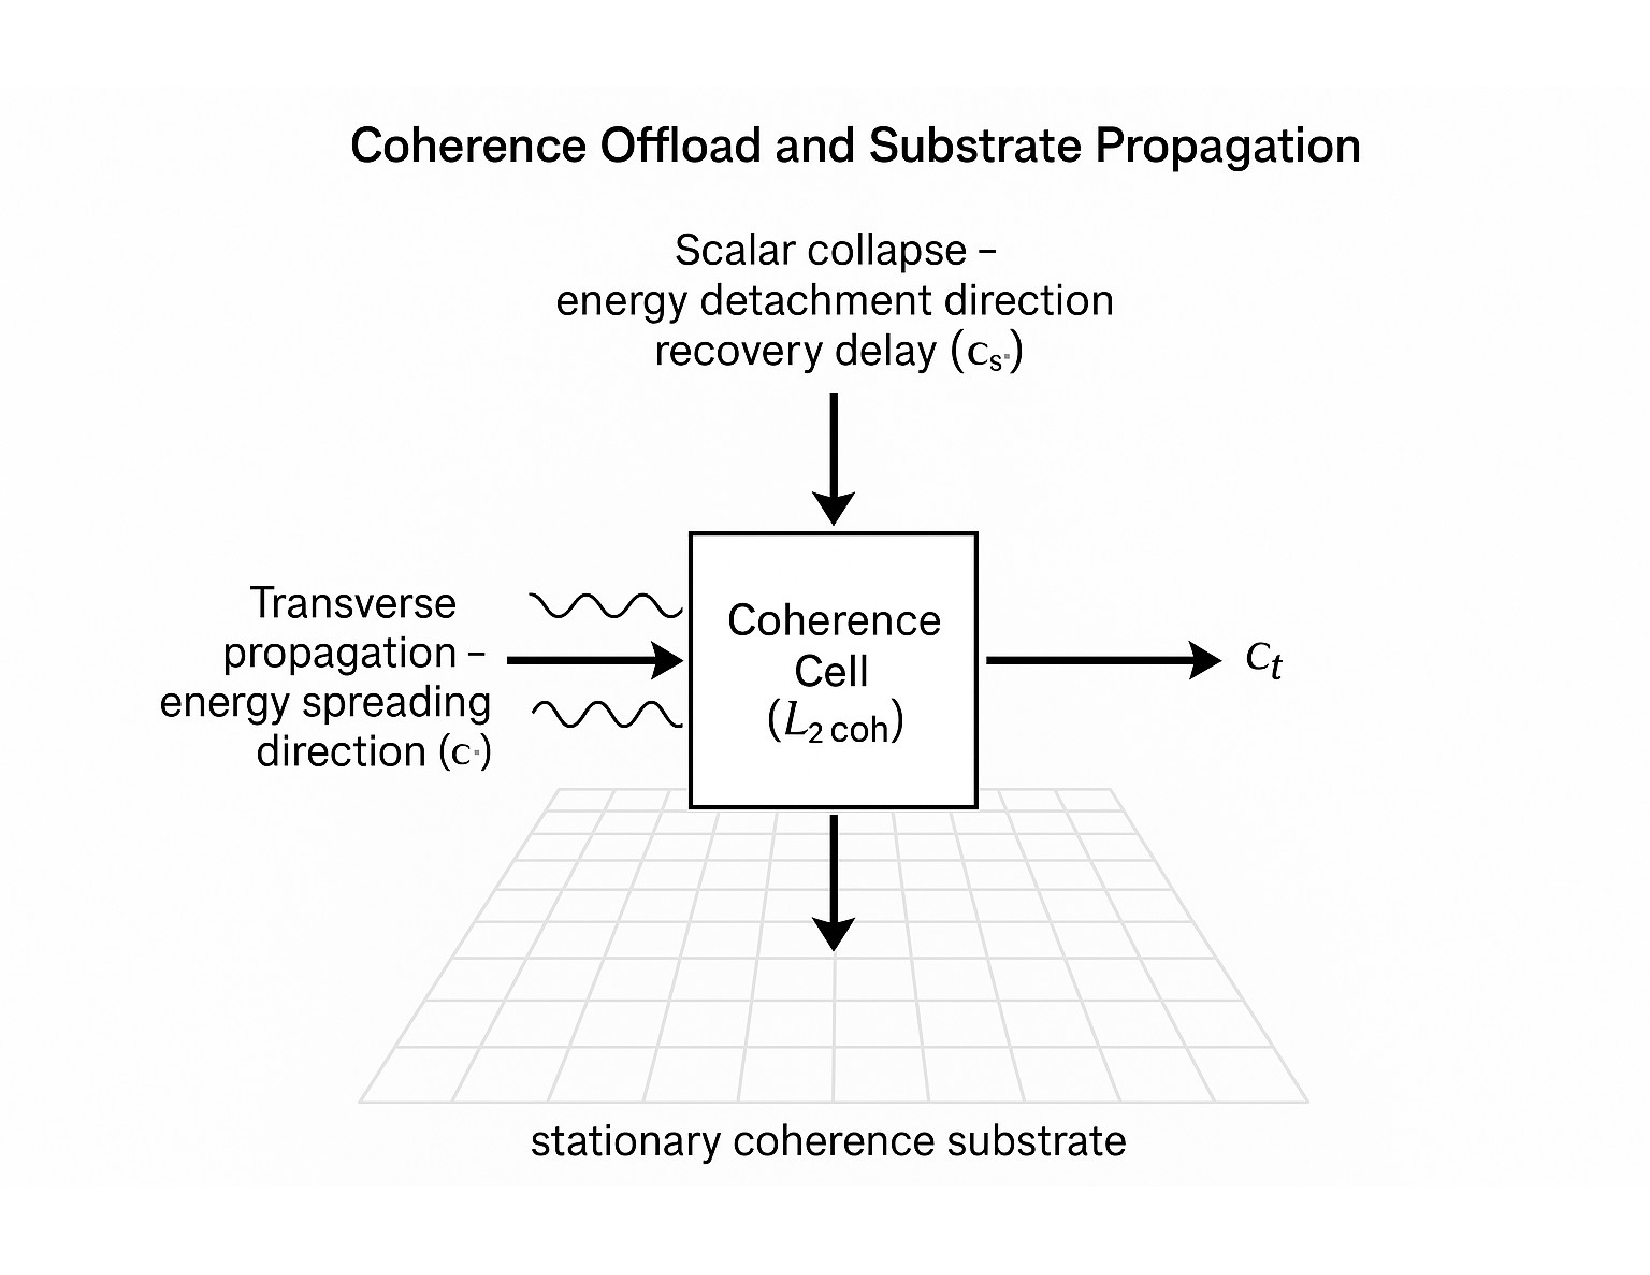
\includegraphics[width=0.9\textwidth]{figures/qsd_lcohcsct.pdf}
    \caption{Coherence Offload and Substrate Propagation}
    \label{fig:qsd_lcohcsct}
\end{figure}

\section{Dimensional Structure of Powers of \texorpdfstring{$c$}{c}}

In conventional physics, the speed of light $c$ appears in equations not only as a velocity, but as a squared or even higher power term—most famously in $E = mc^2$. These exponents are usually accepted as dimensional necessities rather than indicators of internal structure. In Quantum Substrate Dynamics (QSD), however, each power of $c$ has a direct physical interpretation: powers of $c$ represent structured combinations of coherence propagation modes within the substrate.

We begin by examining $E = mc^2$. In standard relativity, this expression relates rest mass to energy, with $c^2$ acting as a conversion factor. But in QSD, this relationship becomes physically meaningful:

\[
E = m \cdot c_s \cdot c_t
\]

Here, $c_s$ is the scalar mode velocity—representing the collapse speed of the coherence envelope during offload—and $c_t$ is the transverse propagation velocity—representing how the released energy spreads across the substrate. Thus, $c^2 = c_s \cdot c_t$ is not an abstract square, but a mode product. It encodes the physical interaction between scalar collapse and transverse distribution: energy release only occurs when these two substrate behaviors act in tandem.

We extend this principle to higher powers of $c$. In QSD, dimensional constructs such as $c^3$, $c^4$, $c^5$, and $c^7$ appear not as dimensional artifacts, but as higher-order coherence flux descriptors.

\begin{table}[ht]
\centering
\caption{Physical Interpretation of Powers of \( c \) in Quantum Substrate Dynamics}
\label{tab:c-powers}
\renewcommand{\arraystretch}{1.3}
\begin{tabular}{|c|c|c|p{8.5cm}|}
\hline
\textbf{Power} & \textbf{Units} & \textbf{QSD Mode Decomposition} & \textbf{Physical Interpretation} \\
\hline
\ensuremath{c} & \ensuremath{\text{L/T}} & \ensuremath{c_t} & Maximum transverse coherence propagation speed; sets local lightcone in coherence-neutral domains. \\
\hline
\ensuremath{c^2} & \ensuremath{\text{L}^2/\text{T}^2} & \ensuremath{c_s \cdot c_t} & Energy–tension conversion factor; scalar collapse $\times$ transverse spread. Appears in $E = mc^2$. \\
\hline
\ensuremath{c^3} & \ensuremath{\text{L}^3/\text{T}^3} & — & Volumetric coherence flow rate; describes how quickly coherence fills a 3D region per time. \\
\hline
\ensuremath{c^4} & \ensuremath{\text{L}^4/\text{T}^4} & \ensuremath{c_t^4} & Transverse energy throughput capacity; a measure of wavefront propagation power during offload. \\
\hline
\ensuremath{c^5} & \ensuremath{\text{L}^5/\text{T}^5} & \ensuremath{c_t^4 \cdot c_s} & Maximum substrate energy throughput rate; appears in the Planck time expression and $\hbar$ derivation. \\
\hline
\ensuremath{c^7} & \ensuremath{\text{L}^7/\text{T}^7} & \ensuremath{c_t^6 \cdot c_s} & Planck pressure numerator; defines the substrate’s yield tension rate in fully saturated regions. \\
\hline
\end{tabular}
\end{table}

Each of these power terms plays a role in substrate-limited physical behavior. For instance, $c^5$ appears in the denominator of the Planck time:

\[
t_P = \sqrt{\frac{\hbar G}{c^5}}
\]

which, when decomposed via QSD, expresses the fastest possible coherent offload interval allowed by the substrate. In this framing, $c^5$ represents the volumetric rate at which energy can be transferred outward, constrained by both scalar initiation and transverse flow.

These structured powers of $c$ are not numerological curiosities—they are the backbone of quantization limits. They encode substrate performance envelopes, and their products with other terms like $G$, $\hbar$, or $L_{\text{coh}}$ reflect the real behavior of offload, delay, and curvature response.

In the following section, we use these decompositions to derive Planck’s constant directly from substrate behavior, showing how it arises from coherent interaction geometry—not as an imposed constant, but as an emergent structural ratio.

\section{First-Principles Derivation of Planck’s Constant}

In this section, we derive Planck’s constant $\hbar$ as an emergent quantity from substrate behavior using Quantum Substrate Dynamics (QSD). The derivation builds on three structural properties introduced in previous sections:

\begin{enumerate}
    \item The substrate supports two orthogonal coherence propagation modes: scalar collapse speed ($c_s$) and transverse spread speed ($c_t$) Fig. \ref{fig:qsd_lcohcsct},
    \item Energy can only be released in full coherence cycles across a fixed geometric region of area $L_{\text{coh}}^2$,
    \item The substrate exhibits curvature compliance, denoted by $G$, representing how easily it distorts under coherence tension.
\end{enumerate}

We begin with the standard Planck time expression:
\[
t_P = \sqrt{\frac{\hbar G}{c^5}}
\]
This equation is traditionally treated as a dimensional curiosity, constructed to combine $\hbar$, $G$, and $c$ into a natural time unit. In QSD, however, this equation takes on direct structural meaning.

First, we decompose $t_P$ based on substrate behavior. Since scalar coherence propagation determines how long it takes the substrate to recover after an offload event, the Planck interval is interpreted as the time required for a scalar wave to traverse a coherence cell:
\[
t_P = \frac{L_{\text{coh}}}{c_s}
\]
Squaring both sides gives:
\[
t_P^2 = \frac{L_{\text{coh}}^2}{c_s^2}
\]

We also decompose $c^5$, which appears in the denominator of the original Planck time equation, into its modal components:
\[
c^5 = c_t^4 \cdot c_s
\]

Substituting these expressions into the Planck time definition:
\[
\frac{L_{\text{coh}}^2}{c_s^2} = \frac{\hbar G}{c_t^4 \cdot c_s}
\]

Solving for $\hbar$:
\[
\hbar = \frac{c_t^4}{c_s} \cdot \frac{L_{\text{coh}}^2}{G}
\]

This expression gives Planck’s constant as a structured ratio of physical substrate quantities:

\begin{itemize}
    \item $c_t^4$ reflects the volumetric coherence spread rate per offload event,
    \item $c_s$ governs how fast energy can be released—setting a timing bottleneck,
    \item $L_{\text{coh}}^2$ defines the minimum area over which a coherent energy transfer must occur,
    \item $G$ characterizes the substrate’s resistance to curvature under stress.
\end{itemize}

Planck’s constant is thus not a fundamental constant in the axiomatic sense, but a derived quantity that encodes the substrate’s ability to cycle coherence through a physical region at a finite rate. It arises from a balance between energy throughput (transverse spread), timing (scalar recovery), geometric constraints (coherence area), and curvature response (substrate compliance).

This derivation confirms that the quantum of action is not an imposed constraint, but a physically emergent limit on how much energy can be released per coherence cycle within a reconfiguring medium. It also provides the structural basis for quantization, as the minimum action associated with a full offload event is determined by these underlying substrate properties.

\section{Physical Interpretation of the Derivation}

The result obtained in Section 4 expresses Planck’s constant as a structured ratio of substrate mode behavior, spatial coherence geometry, and curvature compliance:
\[
\hbar = \frac{c_t^4}{c_s} \cdot \frac{L_{\text{coh}}^2}{G}
\]
This formulation reveals several important physical insights that challenge and refine conventional views of quantization, energy transfer, and temporal evolution. See Fig. \ref{fig:qsd_lcohcsct}.

\subsection{Quantization as a Coherence-Cycle Constraint}

In this framework, quantization arises not from postulated discreteness or operator formalism, but from a physical limitation: the substrate can only offload energy in complete coherence cycles. The transverse mode ($c_t$) governs how quickly coherence energy can spread through a region, but the scalar mode ($c_s$) sets how often such a transfer can occur. This scalar recovery interval creates a natural pacing mechanism: energy cannot be released again until the substrate has completed its prior offload and returned to a stable configuration.

The term $L_{\text{coh}}^2$ defines the minimum spatial area over which a coherent offload can occur. Any emission must span this region; the substrate does not support partial-wave transfers. This establishes $\hbar$ as the smallest unit of coherent action supported by the substrate in both space and time. This behavior is visually confirmed in the simulation presented in Appendix \ref{app:qsd_sim}, which shows discrete emission intervals and mode-separated propagation arising solely from structural substrate pacing.

\subsection{Time as Scalar Recovery Interval}

In QSD, time is not a universal parameter or background stage. It emerges from the rhythmic recovery of the substrate following offload events. The scalar mode defines how fast the substrate can restore phase tension after emission. This rate-limited return process is what defines the Planck interval:
\[
t_P = \frac{L_{\text{coh}}}{c_s}
\]
Accordingly, the passage of time is tied directly to the dynamics of substrate reconfiguration. This explains why energy cannot be released continuously or arbitrarily fast, even in highly energetic systems. The substrate imposes a built-in delay between offload events, thereby structuring both quantization and causality.

\subsection{Causality and Offload Timing}

In conventional relativistic frameworks, causality is preserved by ensuring no signal travels faster than $c$. In QSD, causality is instead enforced by the substrate’s offload rhythm: no energetic event can propagate before the scalar mode has completed a full coherence reset. This creates a deeper, physically grounded boundary on causal interaction. Rather than being merely geometric (lightcones), causality is enforced by energy throughput limits and coherence recovery pacing.

Importantly, this formulation preserves Lorentz invariance: the transverse mode $c_t$ continues to define the observable lightcone in low-curvature domains. However, by linking causality to scalar recovery rather than coordinate time, this model explains why quantized emissions are temporally discrete and globally consistent.

\subsection{Constants as Structured Ratios}

This interpretation shows that Planck’s constant is not a fundamental number of nature inserted to make equations work. Instead, it is a structured ratio:
\[
\hbar = \frac{\text{transverse coherence power}}{\text{scalar recovery rate}} \times \frac{\text{geometric span}}{\text{curvature compliance}}
\]
It encodes the substrate’s capacity to emit energy per coherence cycle, factoring in how fast it can offload, how much it can handle at once, and how long it takes to reset.

This not only provides a physical explanation for why $\hbar$ has its observed value, but also why it is universal across all systems that interact through coherent wave exchange. It further suggests that if the substrate geometry, $c_s$, or $G$ were to vary—such as in high-curvature or early-universe domains—$\hbar$ could shift as well, though such effects would be extraordinarily rare or suppressed under normal conditions.

\subsection{Planck Time as a Substrate Recovery Interval}

In standard dimensional analysis, Planck time is defined as
\[
t_P = \sqrt{\frac{\hbar G}{c^5}} \approx 5.39 \times 10^{-44} \, \text{s}
\]
and is often interpreted as the smallest meaningful interval of time — a quantum gravity limit. However, this view lacks a mechanistic interpretation for why this time is fundamental, or what process enforces it.

In QSD, this same quantity emerges from a different origin: the scalar recovery speed $c_s$ and coherence scale $L_{\text{coh}}$. After each energy offload event, the substrate must reconfigure to restore coherence before another emission can occur. This recovery is not instantaneous — it proceeds at a finite rate $c_s$. The time required to reset a coherence cell of area $L_{\text{coh}}^2$ is therefore:
\[
t_P = \frac{L_{\text{coh}}}{c_s}
\]

This expression has direct structural meaning: it is the \textit{minimum time between quantized emissions from a coherence-saturated cell}. The substrate cannot emit continuously; it is rhythmically constrained by its own capacity for phase recovery.

Crucially, when we assume that the coherence scale is the Planck length \( (L_{\text{coh}} = \ell_P) \) and that scalar recovery proceeds at the speed of light \( (c_s = c) \), the QSD expression exactly recovers the conventional Planck time (see Appendix \ref{app:planklength} for justification):
\[
t_P = \frac{1.616 \times 10^{-35} \, \text{m}}{3.00 \times 10^8 \, \text{m/s}} \approx 5.39 \times 10^{-44} \, \text{s}
\]

This agreement is not a coincidence — it suggests that the Planck time is not merely a dimensional curiosity, but a real physical limit governed by the substrate’s ability to recover coherence between offload events. In this framing, Planck time becomes the \textit{natural cadence of quantized action} — a structural heartbeat of the substrate, not an abstract boundary.

\subsection{Substrate Analogy for Quantization}

To build intuition for how quantization arises in QSD, consider a coherence cell as a loading dock and emitted energy as a wave packet "truck." After a full emission, the coherence dock is full. No new wave can depart until the previous one clears the zone. 

The scalar recovery speed \( c_s \) governs how quickly the substrate resets — that is, how fast the previous energy packet vacates the emission region (see Fig.\ref{fig:qsd_gap}). Only after this causal clearance can the next coherent wave be formed. 

\begin{figure}[H]
    \centering
    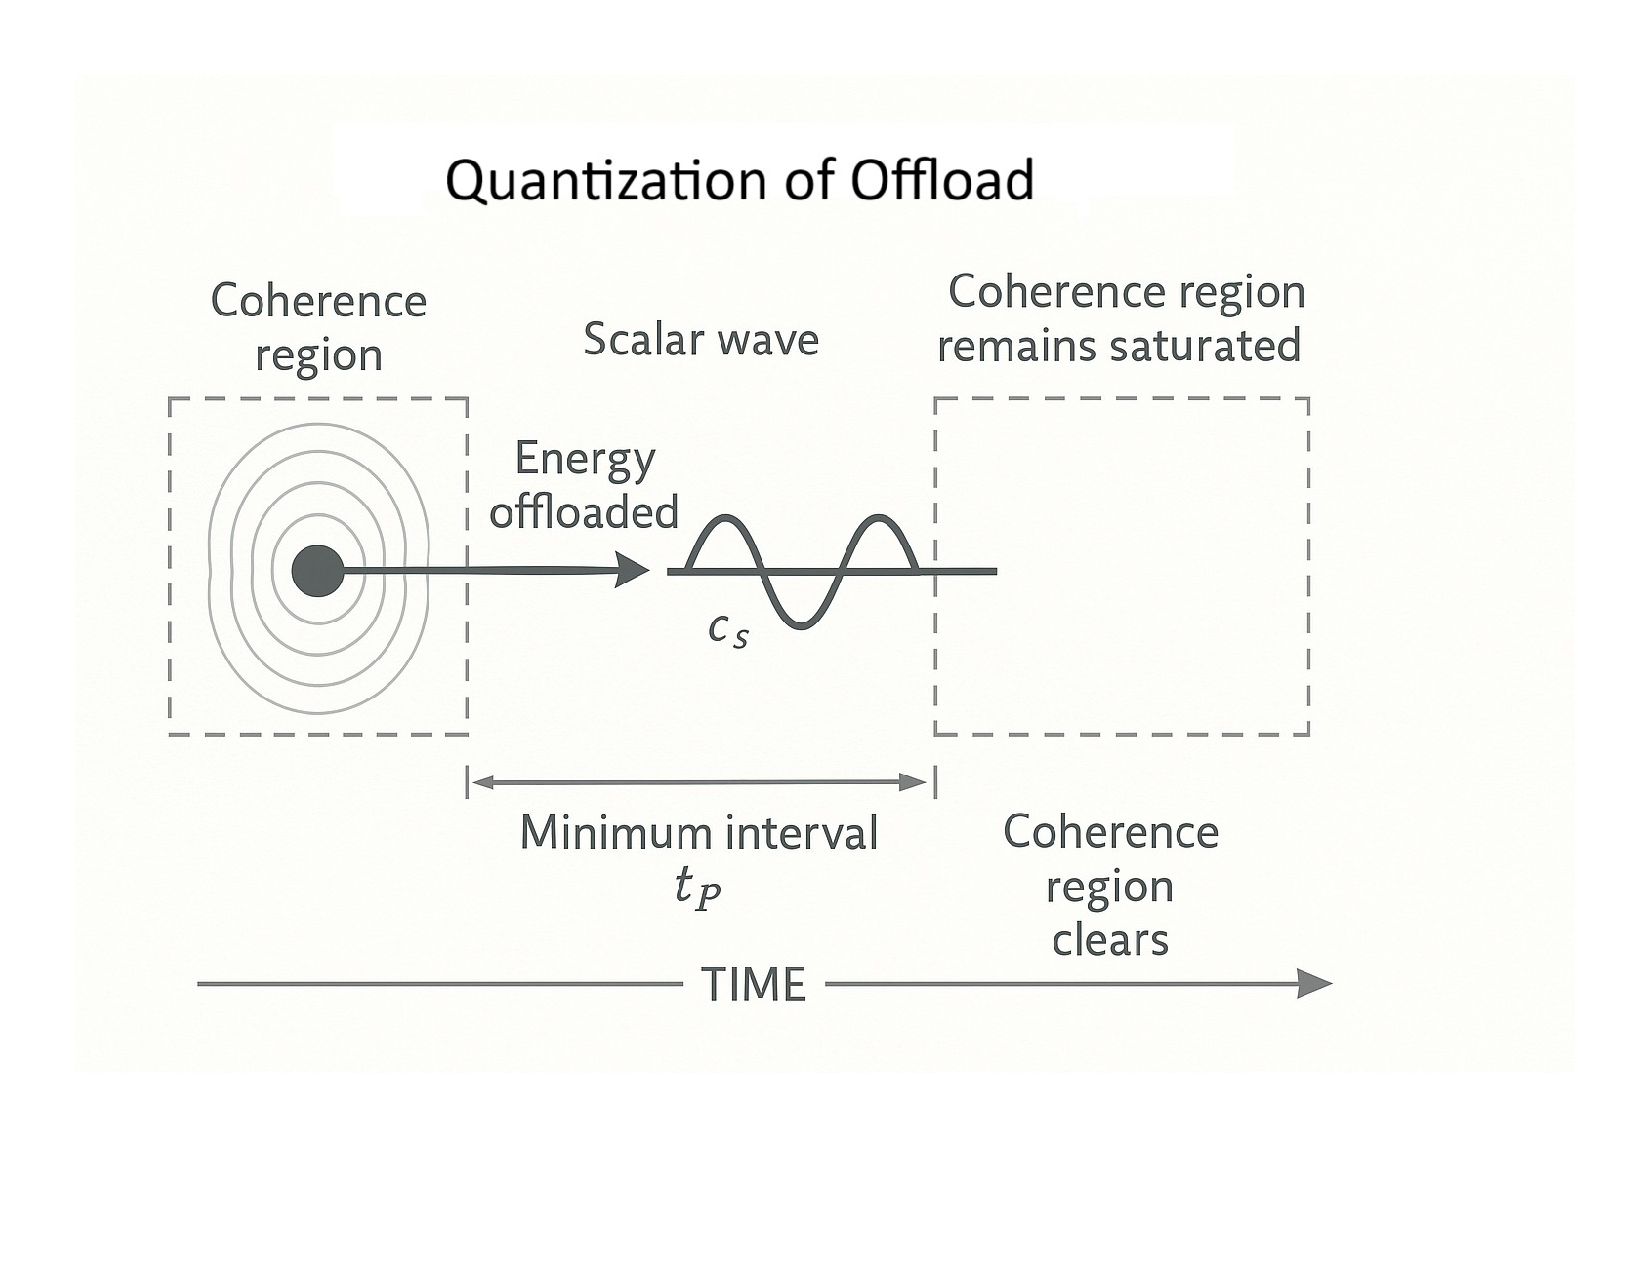
\includegraphics[width=0.8\textwidth]{figures/qsd_quantized_diagram.pdf}
    \caption{Quantization of Offload}
    \label{fig:qsd_gap}
\end{figure}


In this picture, the spacing between emissions is not imposed by a quantum postulate, but is a structural consequence of causal substrate behavior. Quantization, in this view, is not a mystery — it is simply the natural outcome of making space for energy to move.


\section{Consequences and Comparisons}

The derivation of Planck’s constant as a structured consequence of coherence dynamics has far-reaching implications across multiple areas of physics. In this section, we highlight how this framework reinterprets established theories while remaining compatible with known physical behavior.

\subsection{Relation to Canonical Quantum Mechanics}

In conventional quantum mechanics, Planck’s constant is introduced axiomatically. It appears in operator definitions (e.g., $\hat{p} = -i\hbar \nabla$), in the Schrödinger equation, and in quantization rules. Yet none of these formulations explain \textit{why} energy must be transferred in discrete units, or what determines the scale of quantization.

The QSD derivation provides this missing explanation. In this model, $\hbar$ arises as the minimum action required to coherently offload energy through the substrate. The discrete nature of energy levels is not enforced mathematically but emerges from a finite substrate capacity, a real scalar recovery interval, and a coherence-limited transfer envelope. This structural mechanism supports the observed discreteness of quantum transitions, spectral line spacing, and emission timing—without relying on probabilistic postulates or operator algebra.

\subsection{Implications for Quantum Field Theory}

Quantum field theory (QFT) employs $\hbar$ throughout its formalism, particularly in phase-weighted path integrals of the form $e^{iS/\hbar}$. Here, $\hbar$ regulates interference and sets the transition amplitude scale. However, in QFT, the presence of $\hbar$ is again assumed—it is inserted to recover classical behavior in the limit $\hbar \to 0$, but never derived from deeper physics.

In QSD, $\hbar$ is not a tuning knob, but a reflection of how much energy can be coherently transferred per phase-reset cycle. This interpretation suggests that QFT’s structure remains valid under QSD, but that its constants and operator framework should be understood as approximations of a deeper substrate rhythm.

The connection to path integrals becomes clearer: each allowed history in QFT corresponds to a structured coherence evolution that obeys timing constraints set by the substrate. The phase accumulation $S/\hbar$ is thus not an abstract weighting factor, but a normalized action per recovery-limited offload interval. It implies that quantum interference is governed by the substrate’s internal cycle structure, not metaphysical superposition.

\subsection{Contrast with General Relativity}

General relativity (GR) describes spacetime curvature without invoking Planck’s constant. The geometric structure is continuous, and curvature arises from mass-energy via the Einstein field equations. The absence of $\hbar$ in GR reflects its non-quantized nature—but also its incompleteness in describing phenomena where quantization and time intervals matter.

In QSD, curvature compliance $G$ is preserved, but is reinterpreted. It is no longer a measure of gravitational strength, but of how much the substrate resists distortion under coherence tension. This connects mass-energy and curvature through physical substrate behavior. The inclusion of $\hbar$ in the QSD framework makes gravity and quantization part of the same structural continuum.

This approach offers a unified basis for integrating quantum behavior and geometric curvature. Rather than seeking to quantize gravity by discretizing spacetime itself, QSD describes quantization and curvature as co-emergent from substrate properties. Both arise from finite coherence capacity, tension, and reconfiguration delay.

\subsection{Toward Structural Unification}

The reinterpretation of $\hbar$ as a consequence of substrate behavior invites a broader reexamination of other constants and theoretical boundaries. If Planck’s constant emerges from the balance between scalar recovery and transverse flow, then similar reasoning may be extended to:

\begin{itemize}
    \item Boltzmann’s constant $k_B$, as a statistical measure of coherence configuration entropy,
    \item The fine-structure constant $\alpha$, as a dimensionless ratio of offload interaction strength to substrate throughput,
    \item The cosmological constant $\Lambda$, as a large-scale coherence saturation artifact.
\end{itemize}

This opens the door to viewing many “fundamental” constants not as arbitrary inputs but as emergent, structured ratios of deeper substrate mechanics. Future sections of the QSD framework may extend these interpretations, offering predictive unification across quantum, gravitational, thermodynamic, and cosmological domains.

\subsection{Domain Model of Offload Threshold}

The structural origin of Planck’s constant in QSD depends critically on the substrate’s two-mode energy behavior: the distinction between internal mass-lattice absorption and external substrate offload.

At low energies, the substrate’s coherence structure—the mass-phase lattice—can absorb additional energy by increasing internal phase tension, analogous to heating. This energy remains "trapped" within the mass configuration, raising vibrational or structural tension without triggering radiation.

However, once the lattice reaches a saturation threshold, additional energy can no longer be confined internally. At this point, the system transitions into a second domain: coherent offload into the substrate. This occurs via scalar detachment, releasing a complete wavefront into the transverse mode at the earliest available recovery interval.

This behavior can be modeled as a piecewise or threshold-bound process:
\[
E_{\text{total}} =
\begin{cases}
E_{\text{lattice}}(\delta T), & \text{for } T < T_{\text{offload}} \\
\hbar \nu, & \text{for } T \geq T_{\text{offload}}
\end{cases}
\]
Where $T_{\text{offload}}$ represents the structural saturation point of the mass-phase, and $\nu$ is the frequency associated with the offload cycle. Below the threshold, energy changes internal tension; above it, energy must be released externally.

This domain boundary defines the physical origin of quantization: $\hbar$ is not the minimum unit of energy per se—it is the minimum unit that can be offloaded after mass-phase saturation. It is the rate at which the substrate "unpacks" energy after internal capacity is exceeded.

This insight completes the physical interpretation of Planck’s constant: it is not only the result of coherence modes and geometry, but of the structural transition between **energy storage** and **energy release** in a constrained medium. It is the energetic signature of a coherence overload.


\section{Falsifiability and Experimental Predictions}

Although this work presents a theoretical derivation of Planck’s constant from substrate behavior, its assumptions and implications are physically testable. Because the derivation depends on the finite scalar recovery rate and coherence-area geometry of the substrate, it predicts specific constraints on emission timing, energy discretization, and offload dynamics that deviate in detectable ways from standard models under extreme conditions.

\subsection{Emission Delay and Coherence-Rate Saturation}

In QSD, energy offload cannot occur arbitrarily fast. After each emission, the substrate requires a full scalar recovery cycle before another coherent event can occur. This implies that high-frequency emissions—such as those observed in gamma-ray bursts, black hole evaporation, or ultra-intense laser–matter interactions—should exhibit a minimum spacing between quantized emission packets. If these offloads become rate-limited by the scalar mode ($c_s$), we would expect to observe:

\begin{itemize}
    \item Temporal granularity in emission spikes at Planck-scale intervals or their multiples,
    \item Saturation effects at extremely high input energy densities, where further input does not yield more immediate emission.
\end{itemize}

Precision timing in femtosecond or attosecond experiments may be able to probe this floor directly, particularly in high-coherence optical systems or scalar-wave-modulated media.

\subsection{Scalar Precursor Waves and Offload Fronts}

The model predicts that scalar waves are emitted at the boundary of offload events and propagate at the scalar-mode velocity $c_s$, which is distinct from the transverse speed $c_t$ typically associated with light. These scalar waves are not field excitations in the traditional sense, but substrate boundary actions that precede or accompany energy release.

Searches for scalar precursors in astrophysical data—especially those preceding neutrino bursts, core-collapse supernovae, or gravitational wave events—may reveal timing mismatches or early signatures consistent with a coherence-driven offload model. Any deviation from light-speed arrival that precedes high-energy emissions could support the scalar-boundary hypothesis of QSD.

\subsection{Planck Pressure and Yield Limit Observations}

QSD reframes Planck pressure as the maximum yield tension of the substrate: a structural limit beyond which coherent offload fails and permanent curvature collapse occurs (e.g., black holes, phase discontinuities). If this interpretation is correct, systems approaching this pressure should exhibit behavior consistent with coherence saturation:

\begin{itemize}
    \item Suppression of emission,
    \item Transition from discrete to continuous wavefront behavior,
    \item Nonlinear threshold behavior in extreme vacuum energy or early-universe conditions.
\end{itemize}

Observations from black hole thermodynamics, neutron star transitions, or particle accelerator collisions could provide indirect evidence of such saturation regimes.

\subsection{Variation in Substrate Compliance or Geometry}

While the QSD framework predicts that Planck’s constant is universal under typical conditions, it allows the possibility that $\hbar$ could vary in domains where substrate properties deviate significantly. This might occur in regions of extreme curvature (near singularities), at phase boundaries in the early universe, or in hypothetical engineered materials designed to modulate coherence geometry.

If $L_{\text{coh}}$, $c_s$, or $G$ were to vary locally or be modified artificially, we might observe:

\begin{itemize}
    \item Apparent shifts in quantization scale,
    \item Variations in spontaneous emission rates or decay constants,
    \item Anomalous Casimir or vacuum fluctuation effects in substrate-modulating structures.
\end{itemize}

While such effects are not predicted under known conditions, their detection would offer powerful validation of QSD principles.

\subsection{Summary of Falsifiability Criteria}

This derivation of Planck’s constant is falsifiable in multiple ways:

\begin{itemize}
    \item Observation of emissions violating scalar recovery timing would falsify the coherence pacing model.
    \item Absence of full-wave thresholds in high-precision quantum systems would challenge the coherence-cell hypothesis.
    \item Confirmation of scalar-mode emissions arriving ahead of transverse fronts would strongly support the substrate-boundary origin of radiation.
    \item Detection of localized variations in effective $\hbar$ would confirm its dependence on substrate geometry and compliance.
\end{itemize}

Unlike theories that insert $\hbar$ as an assumed universal constant, the QSD framework offers structural predictions that constrain timing, geometry, and propagation behavior. These predictions provide a basis for empirical testing and distinguish QSD as a physically grounded alternative to conventional quantum interpretation.

%%%%%%%%%%%%%%%%%%%%%%%%%%%%%%%%%%%
\section*{Methods}
%%%%%%%%%%%%%%%%%%%%%%%%%%%%%%%%%%%
This manuscript was developed through a combination of theoretical derivation, analytical modeling, and literature-integrated synthesis. The mathematical structures were formulated by the author and refined iteratively to ensure coherence with known physical limits and compatibility with relativistic invariance.

In support of the editorial process, generative AI tools—specifically OpenAI's ChatGPT (version GPT-4o, 2024)—were used to assist in:
\begin{itemize}
    \item Clarifying technical phrasing and improving narrative clarity,
    \item Verifying internal consistency of definitions, terminology, and mathematical structure,
    \item Suggesting appropriate LaTeX formatting and document structuring,
    \item Cross-referencing related scientific concepts to aid contextualization,
    \item Summarizing and formatting external source material already selected by the author.
\end{itemize}

No original theoretical contributions were generated by the AI system; all scientific claims, hypotheses, derivations, and interpretations were authored and reviewed by the human researcher. The use of ChatGPT is disclosed in alignment with journal policy for transparency in the writing process.

%%%%%%%%%%%%%%%%%%%%%%%%%%%%%%%%%%
\section*{Conclusion}
%%%%%%%%%%%%%%%%%%%%%%%%%%%%%%%%%%

This work presents a first-principles derivation of Planck’s constant \( \hbar \) within the framework of Quantum Substrate Dynamics (QSD), demonstrating that what is typically treated as a fundamental constant of nature is instead an emergent property of a finite, conserved coherence substrate undergoing internal reconfiguration.

By modeling mass as a phase-locked coherence structure and energy as the release of stored substrate tension via scalar-mode offload, QSD provides a mechanistic basis for quantization. Planck’s constant arises from this structure as a coherent mode ratio:
\[
\hbar = \frac{c_t^4}{c_s} \cdot \frac{L_{\text{coh}}^2}{G}
\]
Each term in this expression reflects a physically meaningful aspect of substrate behavior: \( c_s \) defines the scalar recovery rate, \( c_t^4 \) represents the transverse coherence throughput, \( L_{\text{coh}}^2 \) specifies the minimum area required for full offload, and \( G \) encodes the curvature compliance of the substrate. Rather than being imposed from outside the theory, these quantities emerge as structural constraints of a conserved medium.

This perspective reframes quantization as a timed, capacity-limited process—not a formal axiom. Energy is not transferred through field lines or point particles, but via local reconfiguration of coherence domains. Discrete emissions, temporal granularity, and causal structure all arise from the finite pacing and geometry of the substrate itself.

In this framing, \( \hbar \) is not a mysterious threshold between classical and quantum domains, but the minimum unit of action permitted by the coherence cycle of a saturated region. Quantization becomes a geometric and dynamic necessity.

By linking \( \hbar \), \( c \), and \( G \) to the same coherence-supporting infrastructure, this derivation lays the groundwork for unifying constants traditionally treated as independent. If modal speeds approach light speed and coherence geometry reduces to the Planck scale, the structure naturally recovers \( \ell_P \) as the smallest support region for a full coherence offload—offering physical meaning to a quantity often treated as a dimensional convenience (see Appendix~A).

Although this analysis is framed in the language of QSD, the resulting expression for Planck’s constant may have broader interpretive value. It provides a physically structured decomposition of \( \hbar \), anchored in mode propagation, geometric support, and curvature response. These insights may inform any theory in which action, causality, or quantization arise from finite coherence behavior.

As such, this work offers not only a theoretical result, but also a practical tool for reinterpreting fundamental constants—and the nature of quantization itself—within both classical and quantum frameworks.



\pagebreak
%%%%%%%%%%%%%%%%%%%%%%%%%%%%%%%%%%%%%%%%%%%%%%%%%%%%%
%%%%%%%%%%%%%%%%%%%%%%%%%%%%%%%%%%%%%%%%%%%%%%%%%%%%%
\section*{Statements and Declarations}
\subsubsection{Funding}  
The author received no financial support for the research, authorship, or publication of this article.
The author has no relevant financial or non-financial interests to disclose.

\subsubsection{Competing Interests}  
The author declares no competing interests.

\subsubsection{Author Contributions}  
The author solely conceived, developed, and wrote the manuscript, including all theoretical content, references, and formatting.

\subsubsection{Data Availability}  
No datasets were generated or analyzed during the current study. All references are publicly available.

\subsubsection{Ethical Approval}  
Not applicable.


\pagebreak
\appendix

%%%%%%%%%%%%%%%%%%%%%%%%%%%%%%%%%%%%%%%%%%%%%%%%%%%%%%%%%%%%%%%%%%%%
% START APPENDIX
%%%%%%%%%%%%%%%%%%%%%%%%%%%%%%%%%%%%%%%%%%%%%%%%%%%%%%%%%%%%%%%%%%%%

%%%%%%%%%%%%%%%%%%%%%%%%%
\section{Possible Identifications of the Coherence Scale \( L_{\text{coh}} \)}
\label{app:planklength}
%%%%%%%%%%%%%%%%%%%%%%%%%

In the main body of this paper, the quantity \(L_{\text{coh}}\) was introduced as the minimum spatial region required to support a full coherent offload cycle within the quantum substrate. This region defines the geometric envelope over which energy can be emitted as a complete coherence packet, and it plays a central role in setting the quantization scale in QSD.

Importantly, this parameter was not assumed to match any known quantum length scale at the outset. Instead, it emerged in the derivation of Planck’s constant as a geometric component in the structural ratio:
\[
\hbar = \frac{c_t^4}{c_s} \cdot \frac{L_{\text{coh}}^2}{G}
\]
However, once the modal speeds are saturated at their relativistic limit (i.e., \(c_s = c_t = c\)), we can rearrange the expression for \(\hbar\) to solve for \(L_{\text{coh}}\):
\[
L_{\text{coh}} = \sqrt{\frac{\hbar G c_s}{c_t^4}} \quad \xrightarrow{c_s = c_t = c} \quad L_{\text{coh}} = \sqrt{\frac{\hbar G}{c^3}} = \ell_P
\]
This result is not an assumption but an outcome: it shows that, under conditions of maximum coherent propagation, the QSD structural scale \(L_{\text{coh}}\) converges precisely to the Planck length \(\ell_P\). In this light, \(\ell_P\) acquires a direct physical meaning as the minimum spatial support required for a full substrate offload — a coherence envelope, not a dimensional artifact.

Other quantum scales, such as the reduced Compton wavelength \(\bar{\lambda}_C = \hbar / (mc)\), may also emerge as byproducts of substrate behavior when specific mass configurations impose tension constraints. However, the Compton scale is mass-dependent, while \(L_{\text{coh}}\) reflects a general substrate property — independent of particle identity.

Thus, rather than presupposing the Planck length, the QSD model recovers it as a natural limiting geometry for coherence-based energy release. This provides a structural interpretation of \(\ell_P\) as the footprint of a complete coherence offload, giving physical substance to a constant traditionally defined by dimensional convenience.

Future work may explore whether other constants can be similarly grounded in substrate geometry and timing.

%%%%%%%%%%%%%%%%%%%%%%%%%%%%
\section{Simulation of Quantized Emission from Scalar Recovery Timing}
\label{app:qsd_sim}
%%%%%%%%%%%%%%%%%%%%%%%%%%%%
To visually demonstrate the structural emergence of quantized offload events in QSD, we implemented a simple discrete simulation. Each coherence cell is modeled as a region that can emit energy only after recovering scalar coherence from a previous offload. The scalar recovery delay, determined by $c_s$, defines a fixed time interval during which no further emission is allowed. This results in rhythmic, discrete emission events spaced by the Planck interval $t_P = L_{\text{coh}} / c_s$.

The figure below shows a grid of coherence cells (rows) evolving over time (columns). Each white square represents a successful offload; black regions indicate recovery lockout. No randomness or quantization rule was imposed — the discrete behavior arises purely from substrate timing structure. This behavior aligns directly with the derived interpretation of $\hbar$ as a structured action interval (see Fig.\ref{fig:qsd_sim}).

\begin{figure}[H]
\label{fig:sim}
    \centering
    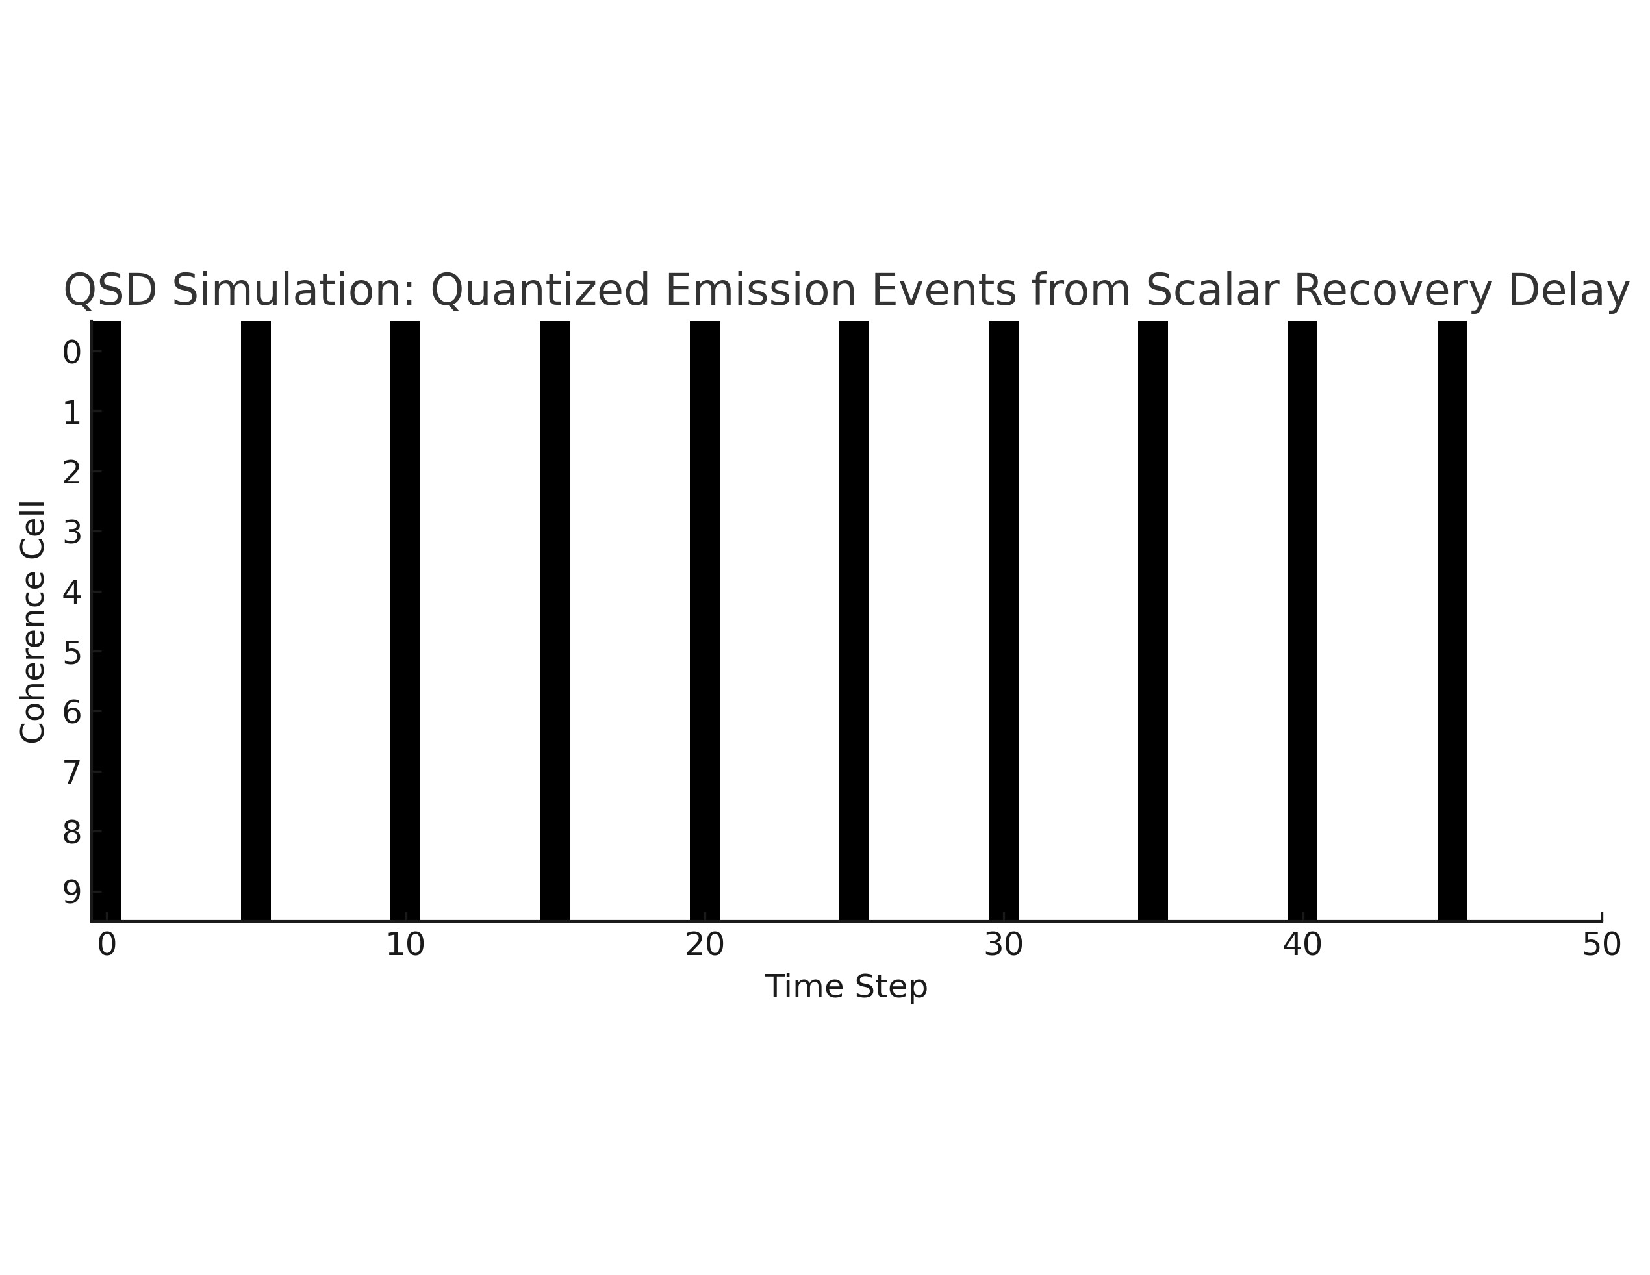
\includegraphics[width=0.8\textwidth]{figures/qsd_quantized_emission.pdf}
    \caption{Simulated coherence cell emissions and transverse wave propagation. Top: Emission events gated by scalar recovery. Bottom: Transverse coherence spreading at speed $c_t$, initiated only after emission. This demonstrates quantization emerging from pacing constraints in QSD.}
    \label{fig:qsd_sim}
\end{figure}



\section{Foundational Shifts in the Physical Interpretation of Planck's Constant}

This appendix summarizes the key theoretical shifts introduced in this work, reframing classical constants and quantum behavior in terms of coherent substrate dynamics.

\begin{table}[h]
\centering
\caption{Twelve Structural Reinterpretations Underlying Planck's Constant in QSD}
\label{tab:foundational-shifts}
\renewcommand{\arraystretch}{1.4}
\begin{tabular}{|c|>{\raggedright\arraybackslash}p{4.2cm}|>{\raggedright\arraybackslash}p{9cm}|}
\hline
\textbf{\#} & \textbf{Concept} & \textbf{Shift Introduced} \\
\hline
1 & \ensuremath{c^2} Decomposition & Reinterpreted as a mode product: \ensuremath{c^2 = c_s \cdot c_t}, representing scalar collapse × transverse spread. \\
\hline
2 & Derivation of \ensuremath{h} & Planck’s constant is re-expressed as a structural ratio: \ensuremath{h = \frac{c_t^4}{c_s} \cdot \frac{L_{\text{coh}}^2}{G}}. \\
\hline
3 & Quantization Origin & Quantization emerges from substrate offload pacing, not imposed discreteness. \\
\hline
4 & Time Redefined & Time is identified as the scalar recovery interval, not a background dimension. \\
\hline
5 & Meaning of \ensuremath{G} & Newton’s constant is reframed as substrate curvature compliance, not gravitational “strength”. \\
\hline
6 & \ensuremath{c^5} Interpreted & Interpreted as the maximum coherent offload throughput of the substrate. \\
\hline
7 & Substrate Is Stationary & All energy transfer occurs through local phase reconfiguration; the field does not move. \\
\hline
8 & Full-Wave Emission & Energy can only be emitted as full coherent wave packets—partial offloads are not permitted. \\
\hline
9 & Scalar Waves & Defined as boundary actions of the substrate, not embedded field modes. \\
\hline
10 & Causality Reframed & Causal structure is defined by scalar return time, not by lightcone alone. \\
\hline
11 & Dimensional Structure & Powers of \ensuremath{c} reflect physical mode combinations, not arbitrary exponentiation. \\
\hline
12 & Constants as Outcomes & \ensuremath{\hbar}, \ensuremath{G}, and \ensuremath{c} are consequences of substrate geometry and capacity—not axioms of the universe. \\
\hline
\end{tabular}
\end{table}



%%%%%%%%%%%%%%%%%%%%%%%%%%%%%%%%%%%%%%%%%%%%%%%%%%%%%%%%%%%%%%%%%%%%
% END APPENDIX
%%%%%%%%%%%%%%%%%%%%%%%%%%%%%%%%%%%%%%%%%%%%%%%%%%%%%%%%%%%%%%%%%%%%


%%%%%%%%%%%%%%%%%%%%%%%%%%%%%%%%%%%%%%%%
%\clearpage
%\bibliography{uqft_references}
%%%%%%%%%%%%%%%%%%%%%%%%%%%%%%%%%%%%%%%%


%%%%%%%%%%%%%%%%%%%%%%%%%%%%%%%%%%%%%%%%%
\clearpage
\begin{thebibliography}{99}
%%%%%%%%%%%%%%%%%%%%%%%%%%%%%%%%%%%%%%%%

\bibitem{bush2025}
\textbf{Preprint.} Bush, M. (2025). Quantum Substrate Dynamics (QSD): A Relativistic Field Model of Emergent Mass, Inertia and Gravity. \textit{Preprints}, 2025060988. \url{https://doi.org/10.20944/preprints202506.0988.v1}

\bibitem{planck1901}
\textbf{Journal article.} Planck, M. (1901). On the Law of Distribution of Energy in the Normal Spectrum. \textit{Annalen der Physik}, 4(553–563). \url{https://doi.org/10.1002/andp.19053221004}

\bibitem{einstein1905} 
\textbf{Journal article.} Einstein, A. (1905). On the electrodynamics of moving bodies. \textit{Annalen der Physik}, 322(10), 891–921. \url{https://doi.org/10.1002/andp.19053221004}

\bibitem{einstein1915} 
\textbf{Journal article.} Einstein, A. (1915). The field equations of gravitation. \textit{Sitzungsberichte der Preussischen Akademie der Wissenschaften}.

\bibitem{sakharov1967} 
\textbf{Journal article.} Sakharov, A. D. (1967). Vacuum quantum fluctuations in curved space and the theory of gravitation. \textit{Soviet Physics Doklady}, 12.

\bibitem{verlinde2011} 
\textbf{Journal article.} Verlinde, E. (2011). On the origin of gravity and the laws of Newton. \textit{Journal of High Energy Physics}, 2011(4), 29. \url{https://doi.org/10.1007/JHEP04(2011)029}

\bibitem{padmanabhan2010}
T.~Padmanabhan, 
\emph{Equipartition of energy in the horizon degrees of freedom and the emergence of gravity}, 
Mod. Phys. Lett. A \textbf{25}(14), 1129–1136 (2010).


\end{thebibliography}


\end{document}

